\section{Density matrix of two energy level system}

\begin{figure}[h!]
	\centering
	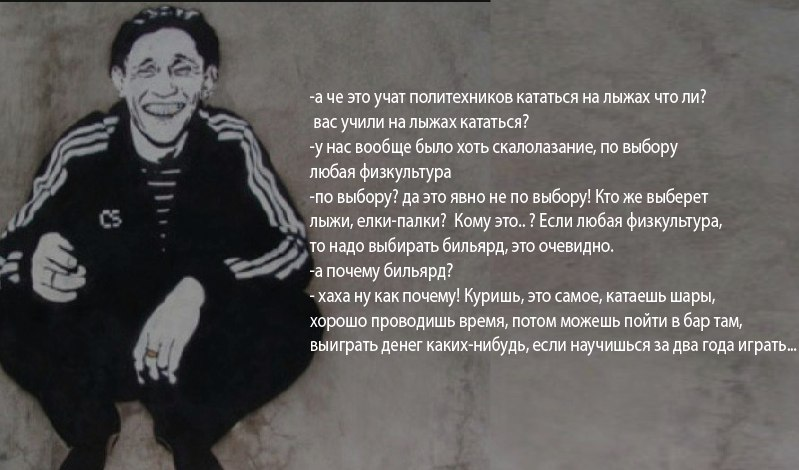
\includegraphics[width=0.8\linewidth]{fig/L4/true_Baiko}
	\caption{The true essence of life choices}
	\label{fig:truebaiko}
\end{figure}

Let consider a two-level system again. In section \ref{sec:atom-field_interaction} we obtained Rabi osculations. Needless to say there weren't any dissipative forces, so turning off the incident field will make the system "freeze" in the last state forever (fig. \ref{fig:turnofffield}). It is obvious that it is not happening in actual truth due to an interaction with immediate media. Adding phenomenological terms to equations for $C_a$ and $C_b$ (e.g. \eqref{eq:rabi_system}) is incorrect because we don't know time dependence of $\ket{\psi(t)}$. The correct way is to use \textit{density matrix formalism}.

\begin{figure}[h!]
	\centering
	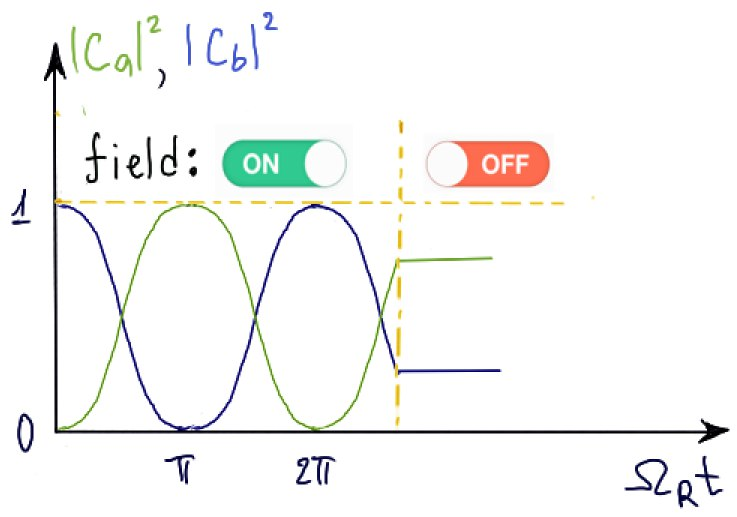
\includegraphics[width=0.65\linewidth]{fig/L5/turn_off_field}
	\caption{Turning the incident field off}
	\label{fig:turnofffield}
\end{figure}


A density matrix is a matrix that describes a quantum system in a mixed state, a statistical ensemble of several quantum states. In other words, density matrix is very useful if we do not know a wave function which contains all the information of the system but we still want to describe our system. There are two possible options (fig. \ref{fig:densmatr}):
\begin{enumerate}
	\item $\ket{\psi_A}$ is known but we need to describe only $B$-system which is intersystem of $A$-system.
	\item $B$ --- is not a conservative system and energy exchanging with reservoir is taking place.
\end{enumerate}
\begin{figure}
	\centering
	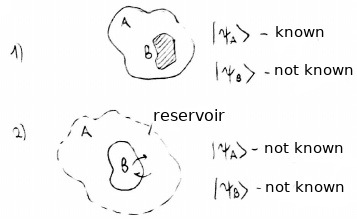
\includegraphics[width=0.7\linewidth]{fig/L5/dens_matr}
	\caption{Possible systems where one need to use density matrix}
	\label{fig:densmatr}
\end{figure}
If $\ket{\psi}$ is known than density matrix is defined by
\begin{equation}
	\boxed{\hat{\rho} = \ket{\psi} \bra{\psi}}
\end{equation}
If we expand to Fock states $\ket{\psi} = \sum C_n \ket{n}$ then 
\begin{equation}
	\hat{\rho} = \sum_{nm} C_n^* C_m \ket{m} \bra{n}.
\end{equation}
Matrix elements --- $\rho_{nm} = C_n^* C_m$.

\begin{testexample}[Density matrix for two-level system.]
	%\textcolor{red}{(UNCOMMENT THIS LATER! (see source))}
	For two-level system we have:
	\begin{equation}
		\ket{\psi} = C_a \ket{a} + C_b \ket{b},
	\end{equation}
	so
	\begin{equation}
		\hat{\rho} = \ket{\psi} \bra{\psi} = 
		\begin{pmatrix}
			\left| C_a (t) \right|^2 & C_a (t) C_b^*(t) \\
			C_b (t) C_a^*(t) & \left| C_b (t) \right|^2
		\end{pmatrix}, \qquad
		\rho_{ij} = \bra{i} \hat{\rho} \ket{j}.
	\end{equation}
\end{testexample}

Mean operator value:
\begin{equation}
	\bar{f} = \bra{\psi} \hat{f} \ket{\psi} \sum_{nm} C_n^* C_m \bra{n} \hat{f} \ket{m} = \sum_{mn} \rho_{nm} f_{nm} = \Tr \left(\hat{\rho} \hat{f}\right).
\end{equation}
\textit{This is the main intended use of density matrix!} Properties:
\begin{enumerate}
	\item Hermiticity: $\hat{\rho}^{\dagger} = \hat{\rho}$.
	\item $\Tr \hat{\rho} = 1 \quad \to \quad$ diagonal elements: $\rho_{mn} = \left| C_n \right|^2$.  Remark: only for pure states!
	\item $]\  \hat{\rho} = \ket{\psi} \bra{\psi} \quad \to \quad \hat{\rho}^2 = \hat{\rho}$. It's easy to show:
	\begin{equation}
		\hat{\rho}^2 = \ket{\psi} \underbrace{\bra{\psi} \ket{\psi}}_{\hookrightarrow = 1} \bra{\psi} = \ket{\psi} \bra{\psi}.
	\end{equation}
	It also means that density matrix of pure state --- projector.
\end{enumerate}

\subsection{Density matrix of mixed state}

Now let us consider a \textit{mixed state}. Let there are lots of systems in different pure states $\ket{\psi_i}$. Let there are $N_i$ particles in $\ket{\psi_i}$, then the whole amount of particles (=systems) is $N = \sum N_i$. The probabily to find any system in $\ket{\psi_i}$ is $\omega_i = \frac{N_i}{N}$. The question we are trying to answer now: how can we find mean operator value?
\begin{equation}
	\bar{f} = \Tr \hat{\rho} \hat{f} = ? \qquad \text{since} \quad \hat{\rho} = ? 
\end{equation}
Scenario is the following:
\begin{enumerate}
	\item Calculation of quantum-average values: $f_i = \bra{\psi_i} \hat{f} \ket{\psi_i}$.
	\item Calculation of classical average values: $\bar{f} = \sum \omega_i f_i$.
\end{enumerate}
So
\begin{multline}
	\bar{f} = \sum \omega_i \bra{\psi_i} \hat{f} \ket{\psi_i} = \sum_i \omega_i \sum_{nm} \underbrace{\left( C_n^i \right)^* C_m}_{\rho_{mn}^i} \underbrace{\bra{n} \hat{f} \ket{m}}_{f_{nm}} = \\
	= \sum_{nm} \sum_i \rho_{mn}^i \omega_i f_{nm} \myeq \Tr \left( \hat{\rho} \hat{f} \right).
\end{multline}
Here we defined density matrix as $\left( \hat{\rho}_{\text{mix}} \right)_{mn} = \sum_i \omega_i \rho_{mn}^i$. Density matrix has a probability meaning:
\begin{equation}
	\hat{\rho}_{\text{mix}} = \sum_i \omega_i \hat{\rho}_i, \qquad \hat{\rho}_i = \ket{\psi_i} \bra{\psi_i}.
\end{equation}
Coefficients $\omega_i$ are defined by \textit{statistical (not quantum!) mechanics} (e.g. Boltzmann distribution).

Remarks:
\begin{enumerate}
	\item $\Tr \hat{\rho}_{\text{mix}} = 1$ by virtue of the fact that $\sum \omega_i = 1$.
	\item $\Tr \hat{\rho}_{\text{mix}}^2 = \sum \omega_i^2 \le 1$. 
	
	Proof:
	\begin{multline}
		\Tr \hat{\rho}_{\text{mix}}^2 = \Tr \sum_{ij} \omega_i \omega_j \sum_{n m} C^*_{m_i} C_{n_i} \ket{n_i} \bra{m_i} \sum_{n' m'} C^*_{m_j'} C_{n_j'} \ket{n_j'} \bra{m_j'} = \\ = \Tr
		\sum_{ij} \omega_i \omega_j \sum_{nmn'm'} C_{m_i}^* C^*_{m_j'}C_{n_i} C_{n_j'} \ket{n_i} \underbrace{\bra{m_i} \ket{n_j'}}_{\hookrightarrow=\delta_{mn'} \delta_{ij}} \bra{m_j'} = \\ = \Tr \sum_i \omega_i^2  \underbrace{\sum_{n'} \left|C_{n'}\right|^2}_{\hookrightarrow = 1} \hat{\rho}_i = \sum_i \omega_i^2.
	\end{multline}
	It means it is not projector anymore! Testing criterion of pureness is introduced by
	\begin{equation}
		\boxed{\mu = \Tr \hat{\rho} - \Tr \hat{\rho}^2 \ge 0}
	\end{equation}
\end{enumerate}

\subsection{Subsystem density matrix}

Let $\hat{f}_A$ is an operator that acts only in subsystem $A$. Now let us ask a question: how to find mean value $\bar{f}_A$?

Subsystem $A$ does not have its own wave function and $\ket{\psi}$ (wave function of $A + B$) does not fall in multiplication of $\ket{\psi_A}$ and $\ket{\psi_B}$. But we can write an expansion in eigenfunctions $\ket{n}$ of subsystem $A$ and $\ket{\alpha}$ of $B$:
\begin{equation}
	\ket{\psi} = \sum_{n \alpha} C_{n \alpha} \ket{n} \ket{\alpha}.
\end{equation}
Now we can write
\begin{multline}
	\bar{f}_A = \bra{\psi} \hat{f}_A \ket{\psi} = \sum_{n \alpha n' \alpha'} C_{n \alpha} C^*_{n' \alpha'} \bra{\alpha'} \overbrace{\bra{n'} \hat{f}_A \ket{n}}^{f_{n' n}} \ket{\alpha} = \\ =
	\sum_{n \alpha n' \alpha'} C_{n \alpha} C^*_{n' \alpha'} f_{n' n} \underbrace{\braket{\alpha'}{\alpha}}_{\hookrightarrow = \delta_{ij}\alpha \alpha'} = \sum_{n n'} \sum_{\alpha}  C_{n \alpha} C^*_{n' \alpha} f_{n' n} = \sum_{n n'} \left( \hat{\rho}_A \right)_{n' n} f_{n' n}.
\end{multline}
Here we denoted
\begin{equation}
	\left( \hat{\rho}_A \right)_{n' n} = \sum_{\alpha}  C_{n \alpha} C^*_{n' \alpha}
\end{equation}
or in other words
\begin{equation}
	\left( \hat{\rho}_A \right)_{n' n} = \sum_{\alpha = \alpha'} \left( \hat{\rho}_{A+B} \right)_{n \alpha n' \alpha'}.
\end{equation}
In the general case:
\begin{equation}
	\boxed{\hat{\rho}_A = \Tr_B \left( \hat{\rho}_{A+B} \right)}
\end{equation}


\subsection{Density matrix for two-level system}

\begin{figure}[h!]
	\centering
	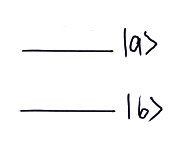
\includegraphics[width=0.25\linewidth]{fig/L4/2lvl}
	\caption{A two-level system}
	\label{fig:2lvl5}
\end{figure}

Let us consider a two-level system with upper state $\ket{a}$ with energy $E_a = \hbar \omega_a$ and lower $\ket{b}$ with $E_b = \hbar \omega_b$. Wave function of such system is
\begin{equation}
	\ket{\psi} = C_a \ket{a} + C_b \ket{b}, \qquad \qquad 
	\ket{a} =
	\begin{pmatrix}
		0\\1
	\end{pmatrix}, \quad
	\ket{b} =
	\begin{pmatrix}
	1\\0
	\end{pmatrix}.
\end{equation}
Density matrix is
\begin{equation}
	\hat{\rho} = 
	\begin{pmatrix}
	\left| C_a (t) \right|^2 & C_a (t) C_b^*(t) \\
	C_b (t) C_a^*(t) & \left| C_b (t) \right|^2
	\end{pmatrix}.
\end{equation}
The von Neumann equation for time evolution
\begin{equation}
	\dot{\hat{\rho}} = - \frac{i}{\hbar} \left[ \hat{\mathscr{H}}, \hat{\rho} \right].
	\label{eq:vonN}
\end{equation}
It is convenient to separate Hamiltonian into two parts $\hat{\mathscr{H}} = \hat{H}_0 + \hat{H}_1$, where
\begin{eqnarray}
	\hat{H}_0 &=& \hbar \omega_a \ket{a} \bra{a} + \hbar \omega_b \ket{b} \bra{b} , \\
	\hat{H}_1 &=& -E(t) \left( d_{ab} \ket{a} \bra{b} + d^*_{ab} \ket{b} \bra{a} \right),
\end{eqnarray}
where $E(t) = E_0 \cos \omega t$. Motion equations
\begin{equation}
	\dot{\rho}_{mn} = - \frac{i}{\hbar} \sum_k \left( H_{mk} \rho_{kn} - \rho_{mk} H_{kn} \right)
\end{equation}
or
\begin{equation}
	\begin{cases}
		\dot{\rho}_{aa} = - \frac{i}{\hbar} E(t) \left( d^*_{ab} \rho_{ab} - d_{ab} \rho_{ba} \right) \\
		\dot{\rho}_{bb} = - \dot{\rho}_{aa} \\
		\dot{\rho}_{ab} = - i \omega_0 \rho_{ab} + i \frac{E(t) d_{ab}}{\hbar} \left( \rho_{bb} - \rho_{aa} \right) \\
		\dot{\rho}_{ba} = \left( \dot{\rho}_{ab} \right)^*
	\end{cases}
	\label{eq:dens_system}
\end{equation}
where $\omega_0 = \omega_a - \omega_b$. Needless to note this is not a RWA yet. Let $\rho_{ab} = \widetilde{\rho}_{ab} e^{-i \omega_0 t}$ then
\begin{multline}
	\dot{\widetilde{\rho}}_{ab} = i \frac{E(t) d_{ab} e^{i \omega_0 t}}{\hbar} \left( \rho_{bb} - \rho_{aa} \right) = i \frac{E_0 d_{ab}}{2 \hbar} \left( e^{i \omega t} + e^{- i \omega t} \right) e^{i \omega_0 t} \left( \rho_{bb} - \rho_{aa} \right) = \\ = \Big/ \omega_0 - \omega \ll \omega_0 \Big/ \approx 
	i \underbrace{\frac{E_0 d_{ab}}{2 \hbar}}_{\Omega_R/2} e^{i \Delta t}\left( \rho_{bb} - \rho_{aa} \right).
\end{multline}
So in RWA we have
\begin{equation}
	\dot{\widetilde{\rho}}_{ab} = i \frac{\Omega_R}{2} e^{i \Delta t} \left( \rho_{bb} - \rho_{aa} \right).
\end{equation}

One may ask a question what are benefits of density matrix formalism? Using such approach we easily "upgrade" \eqref{eq:vonN} by adding dissipation terms. Rules are
\begin{equation}
	\dot{\hat{\rho}} = - \frac{i}{\hbar} \left[ \hat{\mathscr{H}}, \hat{\rho} \right] - \frac{1}{2} \left\{ \hat{\Gamma}, \hat{\rho} \right\},
\end{equation}
where $\Gamma_{mn} = \gamma_{n} \delta_{mn}$, $\gamma_n$ --- rate of dissipation. Why so? It is another long story.

\subsection{Bloch sphere}

It is an easy-to-see way of watching over two-level system. Lets consider density matrix $\hat{\rho}$. First of all, we have only \textit{two independent parameters.} It appears that it is convenient to introduce
\begin{equation}
	\begin{cases}
		x = 2 \Re \rho_{ab} \\
		y = 2 \Im \rho_{ab} \\
		z = \rho_{aa} - \rho_{bb}
	\end{cases}
	\label{eq:tmp_system}
\end{equation} 
One may construct a new vector $\vec{r} = \left\{ x,y,z \right\}$. If $\Tr \hat{\rho} = 1$ then $\left|\vec{r}\right| = 1$, so solutions are placed on a sphere with a unit radius --- \textit{Bloch sphere}.
This vector $\vec{r}$ has a constant axis of rotation $\bm{\Omega}$, in other words
\begin{equation}
	\dot{\vec{r}} = \left[ \bm{\Omega \times \vec{r}} \right].
\end{equation}

Let us consider a specific case: at time $t= 0$ system is in the lower state:
\begin{equation}
	\begin{matrix}
			C_a = 0, & & C_b = 1, \\
		\rho_{bb} \big|_{t=0} = 1, & & \rho_{aa} \big|_{t=0} = 0.
	\end{matrix}
\end{equation}
\begin{figure}[h!]
	\centering
	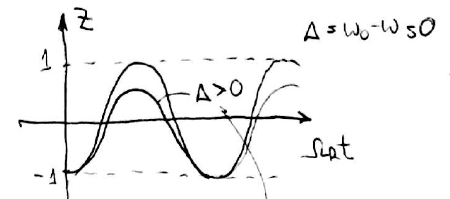
\includegraphics[width=0.6\linewidth]{fig/L5/invers_population}
	\caption{Inverse population of two level system for resonant and non-resonant excitation}
	\label{fig:inverspopulation}
\end{figure}
Let the incident field be $\vec{E} = \vec{E}_0 \cos \left( \omega t + \varphi \right)$. Induced dipole moment is $\vec{d}_{ab} = \bra{a} e \vec{r} \ket{b} \in \mathbb{C}$, so $\left| \bm{\Omega} \right| = \Omega_R = \frac{\vec{E}_0 \cdot \vec{d}_{ab}}{\hbar}$. 

\textit{Remark:} dissipation terms with parameter $\Gamma$ can be easily added to \eqref{eq:tmp_system} (\textcolor{red}{see Scully, find where!}).

\begin{otherlanguage}{russian}
	\begin{hw}[Можно здесь добавить домашку про построение сферы Блоха с затуханием и, например, указать сразу пример системы с $\Gamma \neq 0$.]
		\textcolor{red}{бла бла бла}
	\end{hw}
\end{otherlanguage}


For better understanding we consider a few typical cases: 
\begin{enumerate}
	\item Resonant and non-resonant excitation without dissipation ($\Gamma = 0$). See fig. \ref{fig:bloch1}.
	\begin{figure}[h!]
		\centering
		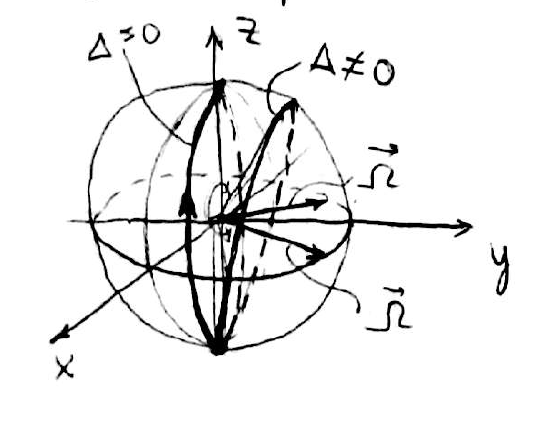
\includegraphics[width=0.7\linewidth]{fig/L5/bloch1}
		\caption{Resonant and non-resonant excitation}
		\label{fig:bloch1}
	\end{figure}
	\item $\Gamma \neq 0$, $\Tr \hat{\rho} = 1$ --- elastic dissipations. See fig. \ref{fig:gammanenol1}.
	\begin{figure}[h!]
		\centering
		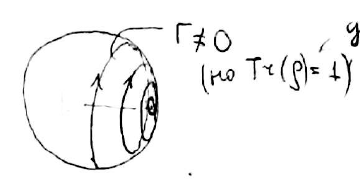
\includegraphics[width=0.6\linewidth]{fig/L5/gamma_ne_nol_1}
		\caption{$\Gamma \neq 0$, $\Tr \hat{\rho} = 1$}
		\label{fig:gammanenol1}
	\end{figure}
	\item $\Gamma \neq 0$, $\Tr \hat{\rho} \neq 1$ --- non-elastic dissipations. See fig. \ref{fig:gammanenol}.
	\begin{figure}[h!]
		\centering
		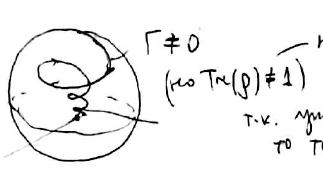
\includegraphics[width=0.6\linewidth]{fig/L5/gamma_ne_nol}
		\caption{$\Gamma \neq 0$, $\Tr \hat{\rho} = 1$. Block sphere ejection}
		\label{fig:gammanenol}
	\end{figure}
	
	
\end{enumerate}
